%*************************************
% ภาคผนวก ข.
%*************************************
\appendixChapterTitle{ข}{การติดตั้งและใช้งาน Ollama}
\vspace*{-0.8in}
\section{การติดตั้งและใช้งาน Ollama}
\hspace*{1.3em}
Ollama เป็น platform สำหรับรัน Large Language Models (LLMs) แบบ local บนเครื่อง PC หรือ Mac รองรับ models หลายตัว เช่น llama, codellama, mistral, gemma\vspace{0.5em}

\begin{mycustomenum2}

\begin{figure}[H]
\centering
\adjustbox{frame, width=1.0\textwidth}{
    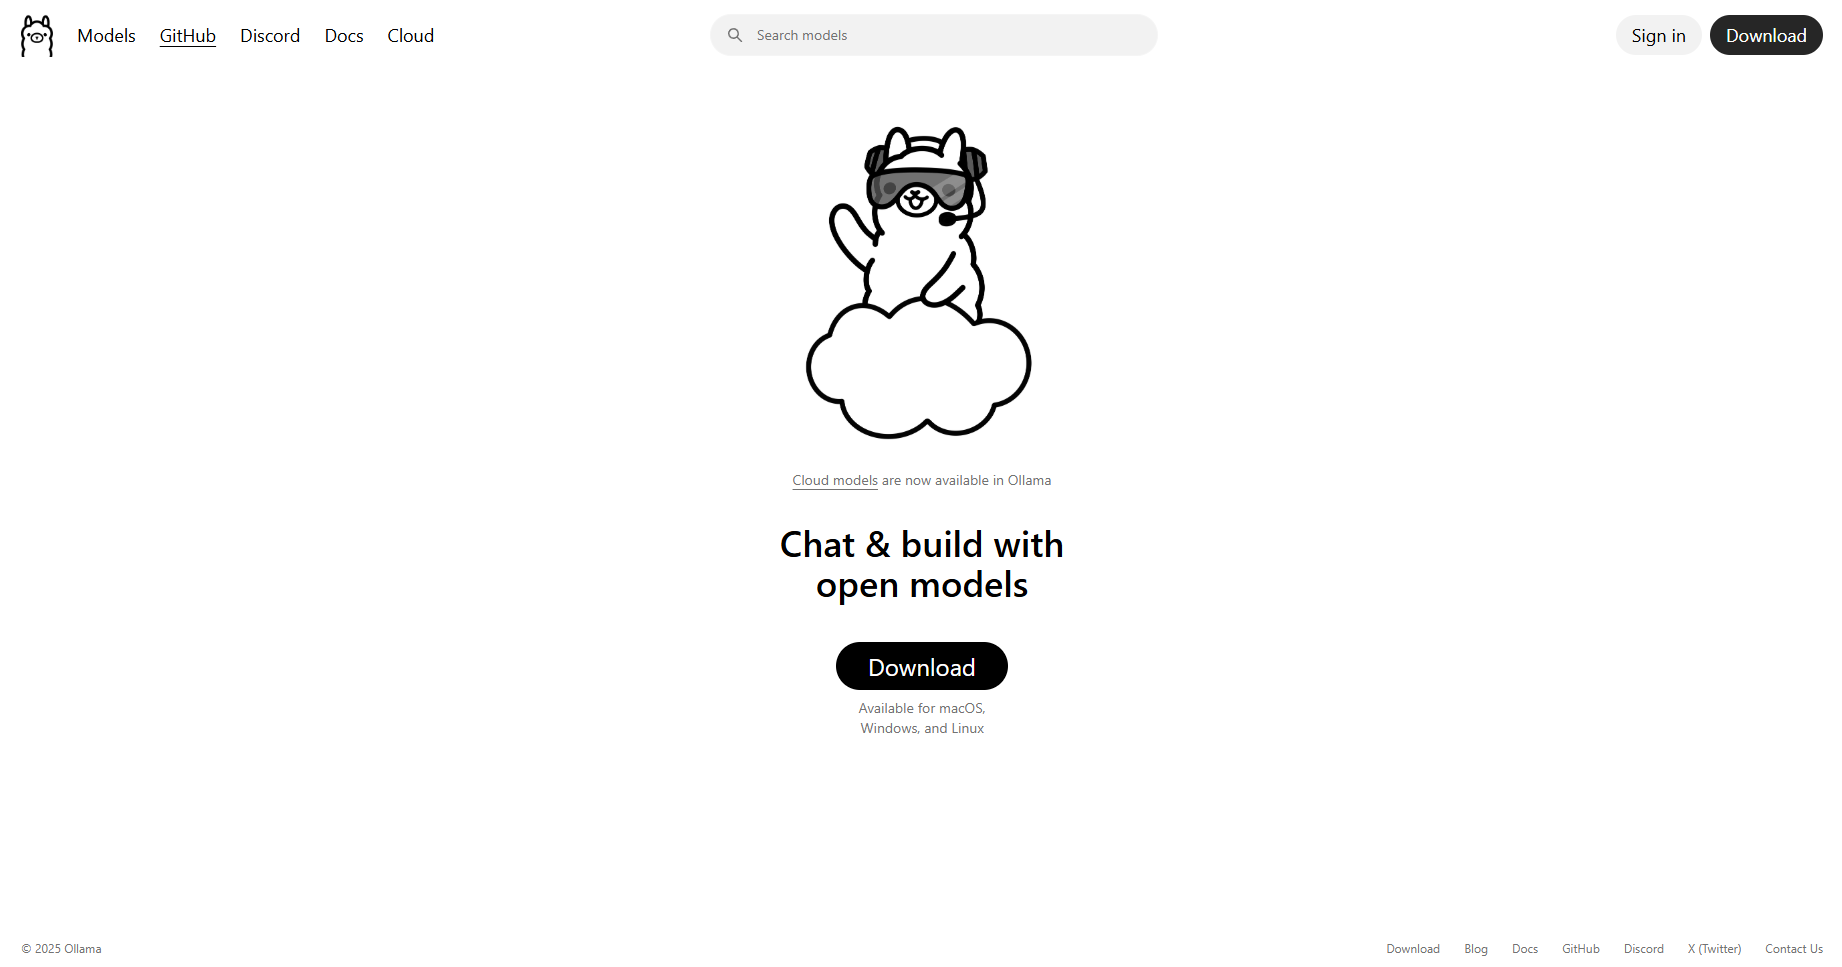
\includegraphics[width=1.0\textwidth]{Image/ollama-page.png}
}
\caption{\fontSixTeen{หน้าแรกของเว็บไซต์ Ollama}}
\label{figB:Ollama1}
\end{figure}
\item ไปที่เว็บไซต์ Ollama (\href{https://www.ollama.com/}{www.ollama.com}) ตัวอย่างหน้าเว็บไซต์ Ollama
\item จากภาพที่ \ref{figB:Ollama1} ให้คลิกที่ \enquote{Download} ก็จะพบกับหน้าจอดังภาพที่ \ref{figB:Ollama2}

\hspace*{1.3em}

\hspace*{1.3em}

\hspace*{1.3em}

\hspace*{1.3em}

\vspace*{-0.6in}
\begin{figure}[H]
\centering
\adjustbox{frame, width=1.0\textwidth}{
    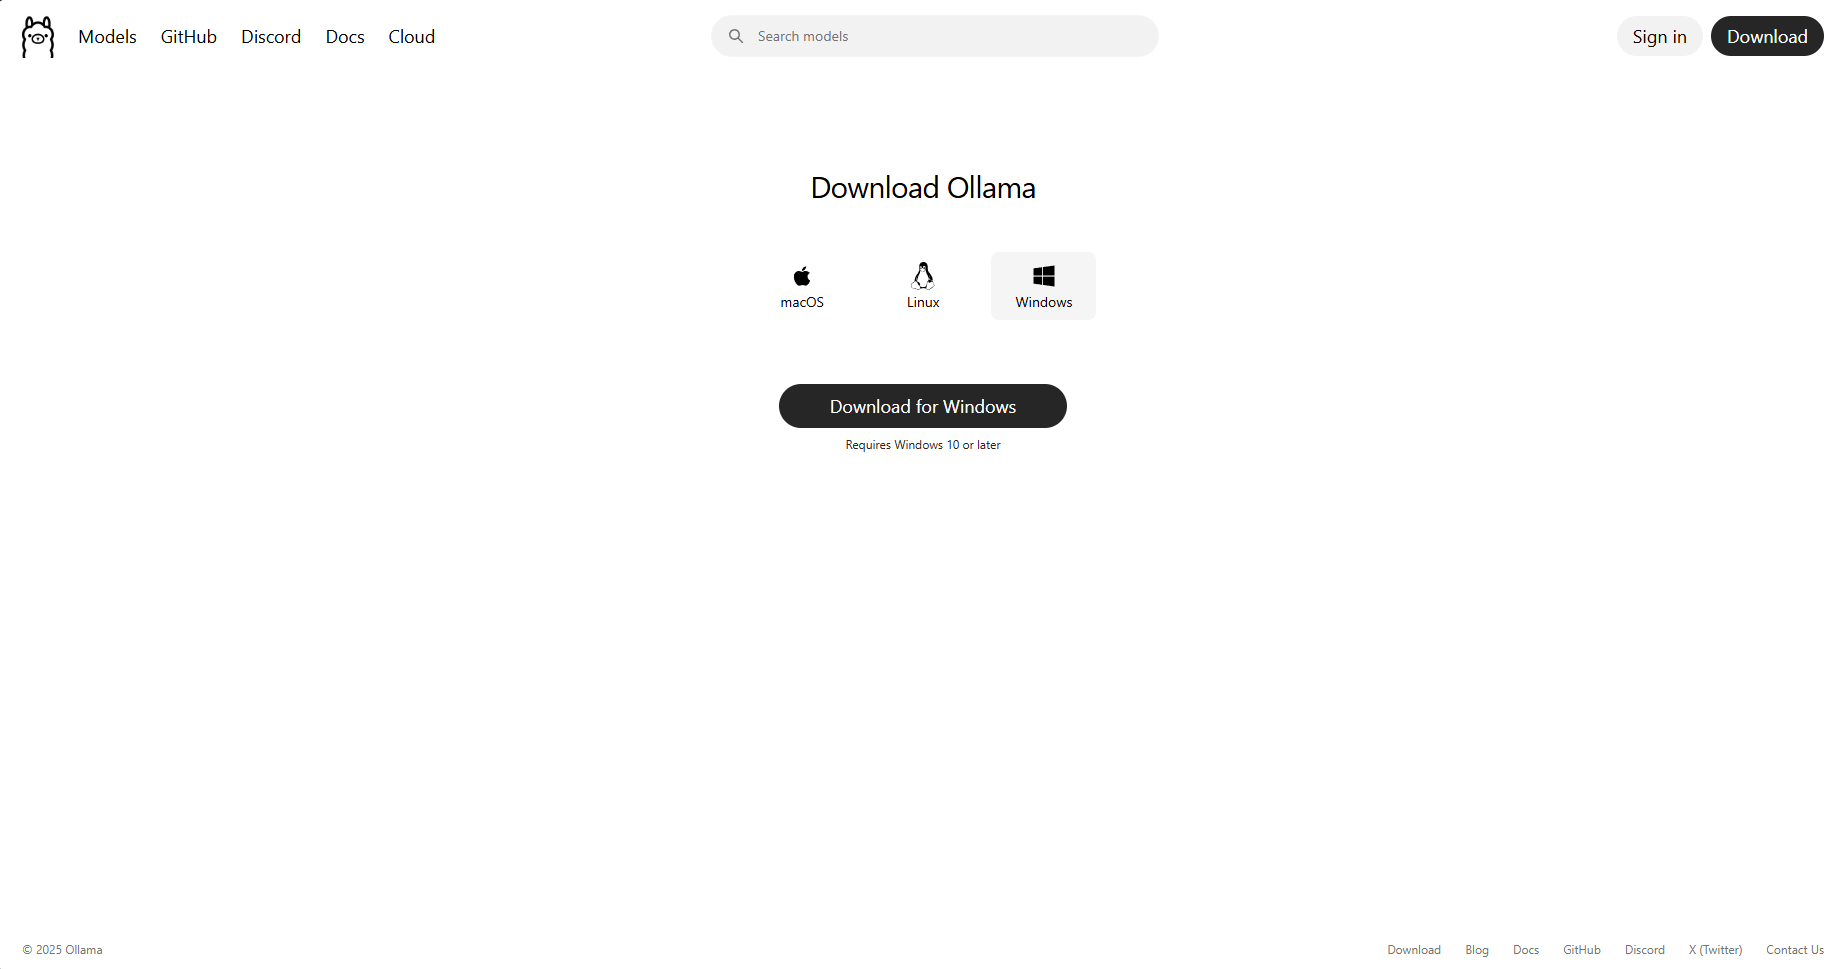
\includegraphics[width=1.0\textwidth]{Image/ollama-page2.png}
}
\caption{\fontSixTeen{หน้าดาวน์โหลด Ollama}}
\label{figB:Ollama2}
\end{figure}
    \item จากภาพที่ \ref{figB:Ollama2} ให้เลือกดาวน์โหลดตัวติดตั้งที่เหมาะสมกับระบบปฏิบัติการของเครื่อง

\begin{figure}[H]
\centering
\adjustbox{frame, width=1.0\textwidth}{
    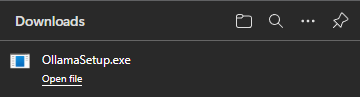
\includegraphics[width=1.0\textwidth]{Image/ollama-page3.png}
}
\caption{\fontSixTeen{ไฟล์สำหรับติดตั้ง Ollama}}
\label{figB:Ollama3}
\end{figure}
    \item จากภาพที่ \ref{figB:Ollama3} ให้ดับเบิ้ลคลิกที่ไฟล์ติดตั้ง Ollama ที่ดาวน์โหลดมา แล้วทำตามขั้นตอนการติดตั้ง

\vspace*{-0.6in}
\begin{figure}[H]
\centering
\adjustbox{frame, width=1.0\textwidth}{
    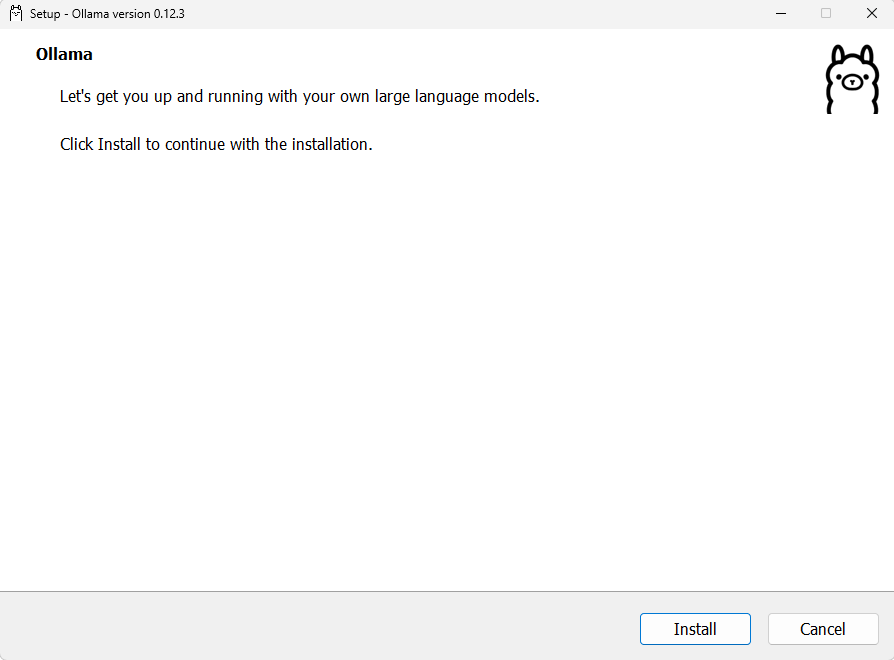
\includegraphics[width=1.0\textwidth]{Image/ollama-page4.png}
}
\caption{\fontSixTeen{หน้าตัวอย่างการติดตั้ง Ollama}}
\label{figB:Ollama4}
\end{figure}
    \item จากภาพที่ \ref{figB:Ollama4} ให้คลิกที่ \enquote{Install} เพื่อเริ่มการติดตั้ง

\vspace*{-0.7in}
\begin{figure}[H]
\centering
\adjustbox{frame, width=1.0\textwidth}{
    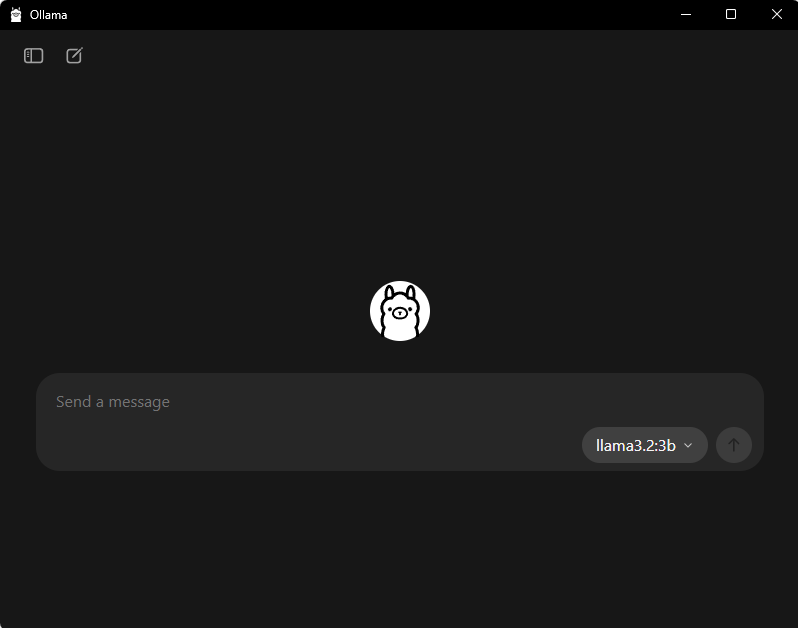
\includegraphics[width=1.0\textwidth]{Image/ollama-page5.png}
}
\caption{\fontSixTeen{หน้าจอหลังติดตั้ง Ollama เสร็จสมบูรณ์}}
\label{figB:Ollama5}
\end{figure}

\vspace*{-0.6in}
\begin{figure}[H]
\centering
\adjustbox{frame, width=1.0\textwidth}{
    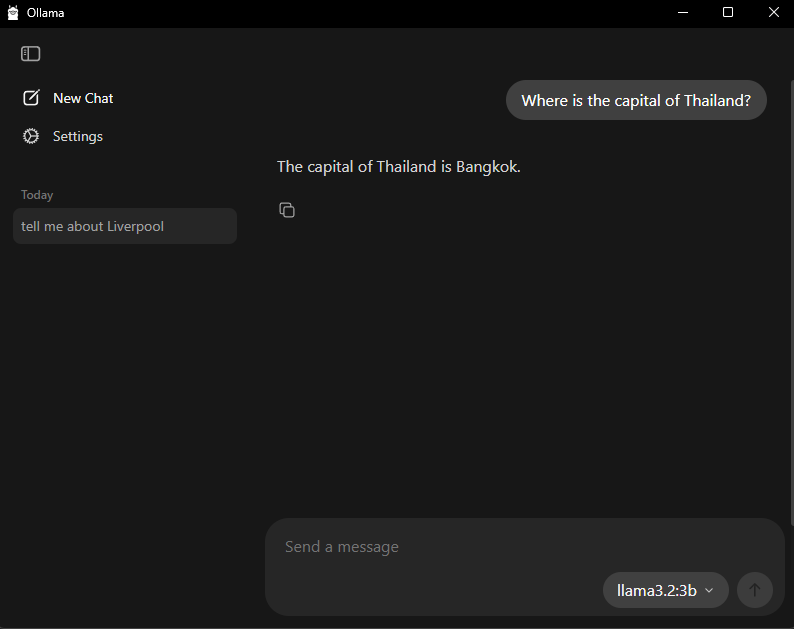
\includegraphics[width=1.0\textwidth]{Image/ollama-page6.png}
}
\caption{\fontSixTeen{หน้าตัวอย่างทดลองการใช้งาน Ollama}}
\label{figB:Ollama6}
\end{figure}

\begin{figure}[H]
\centering
\adjustbox{frame, width=1.0\textwidth}{
    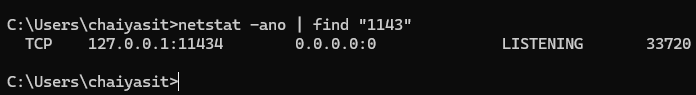
\includegraphics[width=1.0\textwidth]{Image/ollama-page7.png}
}
\caption{\fontSixTeen{หน้าจอตรวจสอบการใช้งานพอร์ต 11434}}
\label{figB:Ollama7}
\end{figure}
\item จากภาพที่ \ref{figB:Ollama7} ตรวจสอบการใช้งานของพอร์ตที่ 11434 ว่าสามารถใช้งานได้หรือไม่ซึ่งเป็นพอร์ตที่ใช้สำหรับการเชื่อมต่อกับ Ollama API

\hspace*{1.3em}

\hspace*{1.3em}

\hspace*{1.3em}

\hspace*{1.3em}

\hspace*{1.3em}

\hspace*{1.3em}

\hspace*{1.3em}

\hspace*{1.3em}

\vspace*{-0.6in}
\begin{figure}[H]
\centering
\adjustbox{frame, width=1.0\textwidth}{
    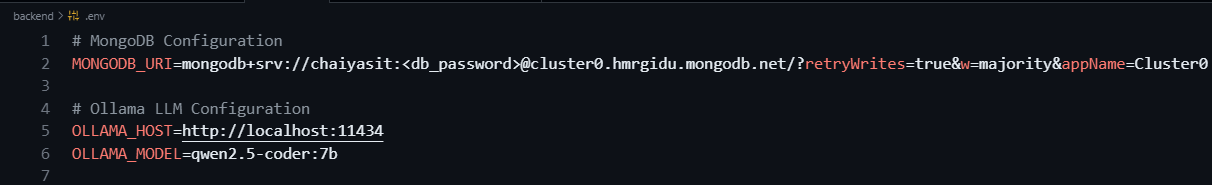
\includegraphics[width=1.0\textwidth]{Image/ollama-page8.png}
}
\caption{\fontSixTeen{หน้าตัวอย่างการนำไปใช้งานกับโปรแกรม}}
\label{figB:Ollama8}
\end{figure}
\item จากภาพที่ \ref{figB:Ollama8} เป็นตัวอย่างการนำ Ollama ไปใช้งานร่วมกับโปรแกรม โดยใช้ Ollama API ในการส่งคำถามและรับคำตอบจากโมเดลที่รันอยู่บนเครื่อง

\end{mycustomenum2}

\hspace*{1.3em}

\hspace*{1.3em}

\hspace*{1.3em}

\hspace*{1.3em}

\hspace*{1.3em}

\hspace*{1.3em}

\hspace*{1.3em}

\hspace*{1.3em}

\hspace*{1.3em}

\hspace*{1.3em}

\hspace*{1.3em}

\hspace*{1.3em}

\hspace*{1.3em}

\hspace*{1.3em}

\hspace*{1.3em}

\hspace*{1.3em}

\hspace*{1.3em}

\hspace*{1.3em}

\hspace*{1.3em}

\hspace*{1.3em}

\begin{center}
\vspace*{-1.5cm}
\textbf{ประวัติผู้จัดทำ}
\end{center}

\vspace{0.5cm} % เพิ่มระยะห่างระหว่างหัวข้อและรูป
% ผู้จัดทำคนที่ 1
\begin{center}
\fbox{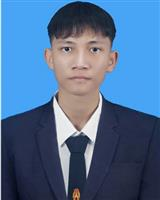
\includegraphics[width=2in,height=2in,keepaspectratio]{Image/profile.jpg}}
\end{center}

\vspace{-0.5cm} % ลดระยะห่างระหว่างรูปและข้อความ

\begin{tabularx}{\textwidth}{lX}
\\
ชื่อ-นามสกุล                    & : นายชัยสิทธิ์ มินทกร
\\
รหัสประจำตัวนักศึกษา           & : 6506022610014
\\
วันเดือนปีเกิด                  & : 4 สิงหาคม พ.ศ.2546
\\
สาขาวิชา                    & : วิศวกรรมสารสนเทศและเครือข่าย 
\\
\\
ประวัติการศึกษา                 
                            & : \hangindent=0.5em
                            จบการศึกษาระดับประถมศึกษา ในปีการศึกษา พ.ศ.2558 \\
                            & ~ \hangindent=0.5em โรงเรียนวัดบางประทุนนอก \\
                            & : \hangindent=0.5em
                            จบการศึกษามัธยมศึกษาตอนต้น ในปีการศึกษา พ.ศ.2561 \\
                            & ~ \hangindent=0.5em โรงเรียนมัธยมวัดสิงห์\\
                            & : \hangindent=0.5em
                            จบการศึกษาประกาศนียบัตรวิชาชีพ ในปีการศึกษา พ.ศ.2564 \\
                            & ~ \hangindent=0.5em สาขาวิชาอิเล็กทรอนิกส์ วิทยาลัยเทคนิคสมุทรสาคร \\
                            & : \hangindent=0.5em
                            ศึกษาต่อในระดับปริญญาตรี ปี พ.ศ.2565 \\
                            & ~ \hangindent=0.5em สาขาวิชาวิศวกรรมสารสนเทศและเครือข่าย คณะเทคโนโลยีและการจัดการอุตสาหกรรม \\
                            & ~ \hangindent=0.5em  มหาวิทยาลัยเทคโนโลยีพระจอมเกล้าพระนครเหนือ วิทยาเขตปราจีนบุรี
                            \\
ที่อยู่ที่สามารถติดต่อได้          & : \hangindent=0.5em
                            204/1 ซอยพระรามที่ 2 ซอย 28 แยก 5 เเขวงจอมทอง เขตจอมทอง กรุงเทพมหานครฯ 10150
                            \\
เบอร์โทรศัพท์มือถือ          & : \hangindent=0.5em
                            092-830-2920
                            \\
ที่อยู่อิเล็กทรอนิกส์          & : \hangindent=0.5em
                            chaiyasit.m@email.kmutnb.ac.th
\end{tabularx}

